\documentclass[acmsmall,screen,review,anonymous]{acmart}

%%
%% \BibTeX command to typeset BibTeX logo in the docs
\AtBeginDocument{%
  \providecommand\BibTeX{{%
    Bib\TeX}}}

%% Rights management information.  This information is sent to you
%% when you complete the rights form.  These commands have SAMPLE
%% values in them; it is your responsibility as an author to replace
%% the commands and values with those provided to you when you
%% complete the rights form.
\setcopyright{acmcopyright}
\copyrightyear{2018}
\acmYear{2018}
\acmDOI{XXXXXXX.XXXXXXX}


%%
%% Submission ID.
%% Use this when submitting an article to a sponsored event. You'll
%% receive a unique submission ID from the organizers
%% of the event, and this ID should be used as the parameter to this command.
%%\acmSubmissionID{123-A56-BU3}
\usepackage{multirow}

\begin{document}

\title{Bridging the Gap Between Visual and Analytical Machine Learning Testing}

\author{Anon}

\begin{abstract}
  A clear and well-documented \LaTeX\ document is presented as an
  article formatted for publication by ACM in a conference proceedings
  or journal publication. Based on the ``acmart'' document class, this
  article presents and explains many of the common variations, as well
  as many of the formatting elements an author may use in the
  preparation of the documentation of their work.
\end{abstract}

\maketitle

\section{Introduction}\label{sec:intro}
% what problem are we trying to solve?
% what is our motivation here?

\section{Preliminaries}\label{sec:prelim}
\subsection{Related Work}\label{sec:related}
\subsection{Background}\label{sec:background}
\subsection{Internal Structure of Jupyter Notebooks}\ref{sec:nbformat}
% we need to explain the json structure of jupyter notebooks, we
% reference this in the methodology to explain the github query.
\bibliographystyle{ACM-Reference-Format}
\bibliography{bibliography}

\section{Methodology}\label{sec:method}
% TODO is there a scientific term in SE research to explain reading
% code in detail?
This section presents the methodology used to conduct the empirical
study presented in Section~\ref{sec:intro}. Figure~\ref{fig:method}
presents an overview of all relevant steps used in this study. The
empirical analysis comprises of three distinct phases namely:
\textit{the data collection phase}, \textit{identification of related
visualisation and assertion pairs} and finally a \textit{complete
analysis of the notebooks} to identify the final set of 29
visualisation and assertion pairs.

The yellow boxes in the data collection phase represent filters that
were applied to the 54K notebooks obtained from Gihub, to obtain the
final sample size of 1.7K notebooks used in the empirical study. The
red boxes represent the exclusion criteria used during phase two to
remove notebooks note relevant for this study. Finally, the green
boxes in phase 3 represent the manual analysis conducted to identify
the final 29 visualisation and assertion pairs.

Boxes appearning next to one-another imply that they were applied
using an "OR" operator. While boxes appearning below one-another imply
an "AND" operator. Text in double quotes represent the string pattern
used in the search query.

More details regarding each phase of the methodology is presented below.

\begin{figure}
  \centering
  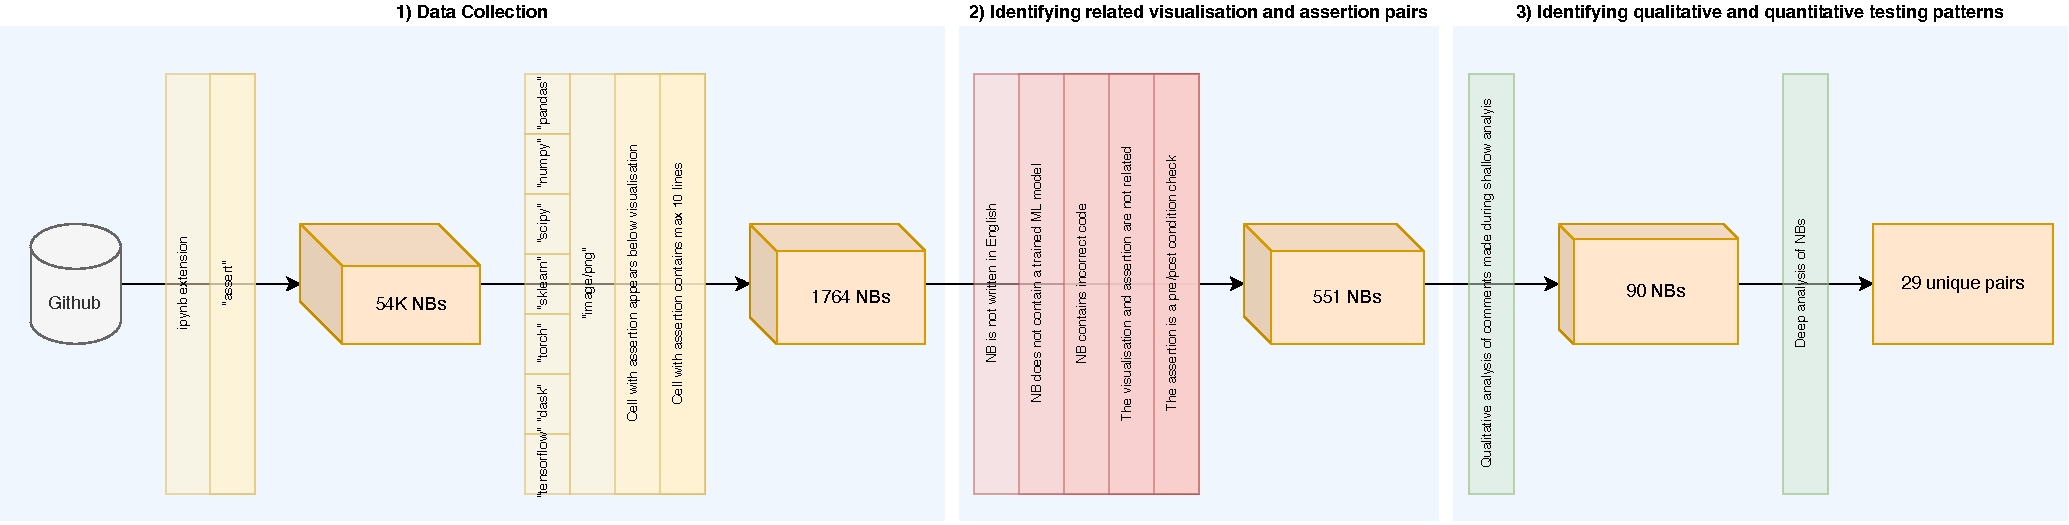
\includegraphics[width=\textwidth]{method.pdf}
  \caption{Methodology used to collect and analyse Jupyter notebooks
    in this study.}
  \label{fig:method}
\end{figure}

\subsection{Data Collection}\label{sec:data-collect}

We mined public repositories from Github to collect Jupyter
notebooks---files with the \texttt{.ipynb} extension---that contain
the keyword ``assert'' in them.

% TODO is it clear what I am trying to say here?
% FIXME is "testing statement" the right terminology?

We intentionally keep the search criteria on Github broad by only
checking for the appropriate filetype and the presence of the
``assert'' keyword. This is because, the ``assert'' keyword is used in
python to define tests. Additionally, popular python libraries which
provide a testing interface (such as nose, unittest and numpy),
contain the same keyword in their API. Thus, our search criteria
captures a large initial sample of $54,070$ notebooks with a variety
of testing statements. Our approach also prevents the need to craft a
custom search query based on an exhaustive list of keywords that
appear in all python testing libraries.

\begin{table}
  \centering
  \caption{Filters used during data collection phase.}
  \begin{tabular}{l p{0.4\textwidth} p{0.4\textwidth}}
    \toprule
    \textbf{ID} &
    \textbf{Filter} &
    \textbf{Rationale}\\
    \midrule
    \emph{\textbf{F1}} &
    Files with extension \texttt{.ipynb} &
    This translates to the following Github search query:
    \texttt{filename:"Jupyter Notebook"}.\\
    \emph{\textbf{F2}} &
    Notebooks with \texttt{"assert"} keyword &
    \texttt{"assert"} is used in python to define tests. Additionally,
    it also appears in other python libraries which provide their own
    testing interface.\\
    \emph{\textbf{F2}} &
    Notebooks with popular data science or machine learning libraries &
    The list of python libraries is derived by performing a web search
    along with the author's prior knowledge and expertise in ML. We
    combine the patterns using an \texttt{"OR"} operator. The final
    regex pattern is the following:
    \texttt{"tensorflow"|"dask"|"torch"|"sklearn"
    |"scipy"|"numpy"|"pandas"}.\\
    \emph{\textbf{F3}} &
    Notebooks that contain visualisations &
    Section~\ref{sec:nbformat} describes the internal json structure
    of Jupyter notebooks. Visualisations are stored as binary strings
    under the \texttt{"image/png"} field.\\
    \emph{\textbf{F4}} &
    Notebooks where the assertion appears below the visualisation &
    The code cell containing the assertion must be defined below the
    cell that produces the visualisation. Any number of markdown cells
    may appear between the visualisation and assertion cells. See
    Section~\ref{sec:cell-arrangement} for detailed explanation.\\
    \emph{\textbf{F5}} &
    Notebooks where the assertion cell is not longer than 10 lines &
    The code cell containing the assertion should not be longer than
    10 lines. The threshold for max lines was derived based on our
    observations from a random sample of 50 notebooks. See
    Section~\ref{sec:cell-arrangement} for detailed explanation.\\
    \bottomrule
  \end{tabular}
  \label{tab:filters}
\end{table}

Table~\ref{tab:filters} summarises the filters used during the data
collection phase to obtain the final sample of 1.7K notebooks from the
initial sample of 54K notebooks mined from Github. The table provides
a short description of the filter along with our rationale for using
them.

% TODO don't mention quantity of random sample; then we need to
% explain/defend this choice
We used an iterative approach to determine the effectiveness of each
filter that was used. We applied each filter in the same order as
presented in Table~\ref{tab:filters}, starting with F1. We randomly
sampled 50 notebooks from the population of notebooks obtained after
applying the filter. We then conduct the qualitative assessment
presented in Section~\ref{REFME} and observe the number of related
visualisation and assertion pairs. In each new iteration, we
progressively add the other filters and include the filter if the
number of relevant visualisation and assertion pairs increases.

\begin{figure}
  \centering
  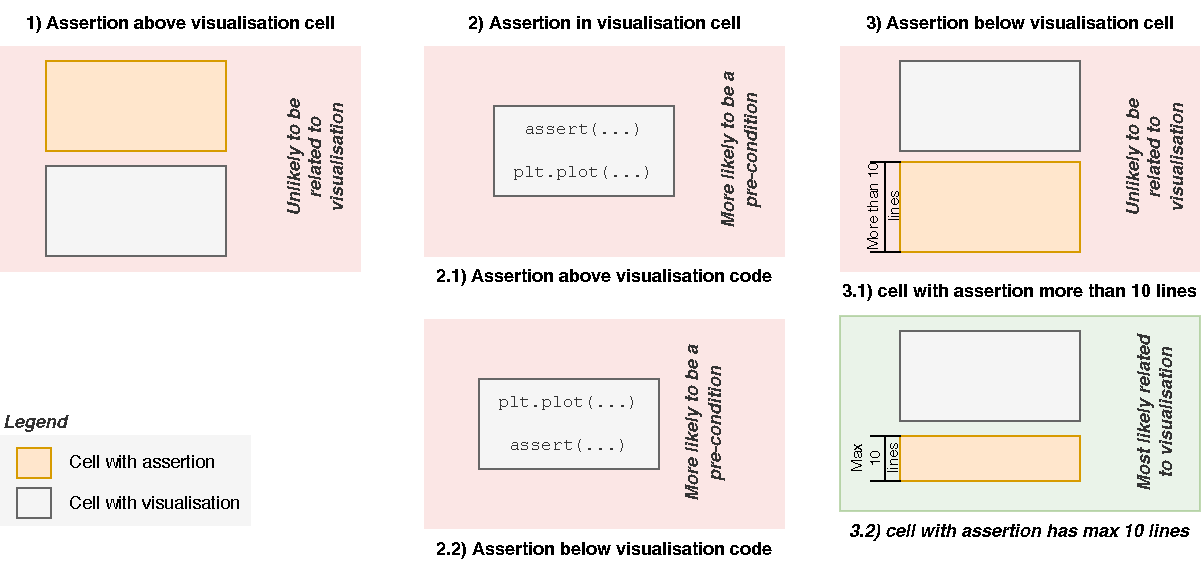
\includegraphics[width=\textwidth]{nb-structure.pdf}
  \caption{Arrangement of code cells containing assertion and
    visualisation.}
  \label{fig:cell-arrangement}
\end{figure}

For RQ1, we are interested in finding empirical evidence of
visualisations and corresponding assertions used in the wild. To
answer this question, we further reduce our notebook sample size by
assuming a specific order in which the visualisation and assertion
code cells appear in the notebooks. Figure~\ref{fig:cell-arrangement}
presents a visual representation of various arrangements of code cells
that may occur in notebooks. Note that the visual representation omits
markdown cells since we only consider the order of code cells in our
analysis. In the actual notebook however, one or more markdown cells
may be present between the visualisation and assertion cells.

As explained above, the selected arrangement of code cells was
discovered by qualitatively analysing a random sample of notebooks
with the code cell arrangements presented in
Figure~\ref{fig:cell-arrangement}. We observed the signal-to-noise
ratio for each cell arrangement. And picked the arrangement with the
least signal-to-noise ratio. Table~\ref{tab:cell-arrangement}
summarises our observations from the various cell arrangements.

\begin{table}
  \centering
  \caption{Observations from random samples of notebooks with various
  cell arrangement.}
  \begin{tabular}{p{0.4\textwidth} p{0.4\textwidth}}
    \toprule
    \emph{\textbf{Cell arrangement}} &
    \emph{\textbf{Observations}}\\
    \midrule
    Assertion above visualisation cell &
    The assertions in this arrangement were typically not related to the visualisation below. Often, a markdown cell present between the assertion and visualisation code cells, would mark the begining of a new section in the notebook. In other cases, the assertions were typically pre-condition checks to ensure that the visualisation code would not encounter any errors. Pre-condition checks typically include checking the shape of features that are used in the visualisation. Or checking that the length of the ``x''and ``y`` features are the same to ensure a continuous line in the plot.\\
    Assertion in the visualisation cell &
    There are two possible scenarios here:
    \begin{enumerate}
    \item[2.1]{This is the first one.}
    \item[2.2]{This is the second one.}
    \end{enumerate}\\

    \bottomrule
  \end{tabular}
  \label{tab:cell-arrangement}
\end{table}

We assume, that the visualisation and assertion pairs of interest, are
more likely to occur in notebooks where the assertion follow

\subsection{Identifying Related Visualisation and Assertion
Pairs}\ref{sec:identify-related-pairs}
% at some point, I think we will have to explain what a
% pre/post-condition check is; then we can ellaborate on our
% experiments with the strictness and proximity of the assert
% statement
% - we have to justify that most of the examples we found when the
% assertion was in the same cell, were pre/post-conditions; whereas
% looking at assertions in the next code cell was more fruitful

\begin{table}
  \centering
  \caption{Exclusion criterion used to reduce sample size of notebooks
    prior to conducting manual analysis to identify related
    visualisation and assertion pairs.}
  \begin{tabular}{l p{0.3\linewidth} p{0.3\linewidth}}
    \toprule
    \textbf{ID} &
    \textbf{Exclusion Criteria(EC)} &
    \textbf{Rationale}\\
    \midrule
    \textbf{EC1} &
    NB does not contain popular data science or machine
    learning libraries &
    \texttt{"pandas|numpy|scipy|sklearn |torch|dask|tensorflow"}\\
    \textbf{EC2} &
    NB does not contain any visualisations &
    TODO\\
    \textbf{EC3} &
    NB conforms to a strict structure as explained in~\ref{REFME} &
    TODO\\
    \bottomrule
  \end{tabular}
  \label{tab:pre-exclusion-criteria}
\end{table}
\subsection{Deeper Analysis of Notebooks}\ref{sec:deep-dive}
\section{Threats to Validity}\ref{sec:threats}
% defend use of github as source for notebooks:
% - why did kaggle not work (refer to notes)
% - why did the existing replication packages not work?

% motivation for keeping the search on github broad:
% - not only does it pick up python assert statements, but also flags
% - notebooks that use other testing libraries or modules that provide a
% - testing interface. This is a good compromise between doing an
% - exhaustive search of all testing method names in the python
% - ecosystem and then doing a search for each of those patterns

\end{document}

